\documentclass[tikz,border=0pt]{standalone}
\begin{document}
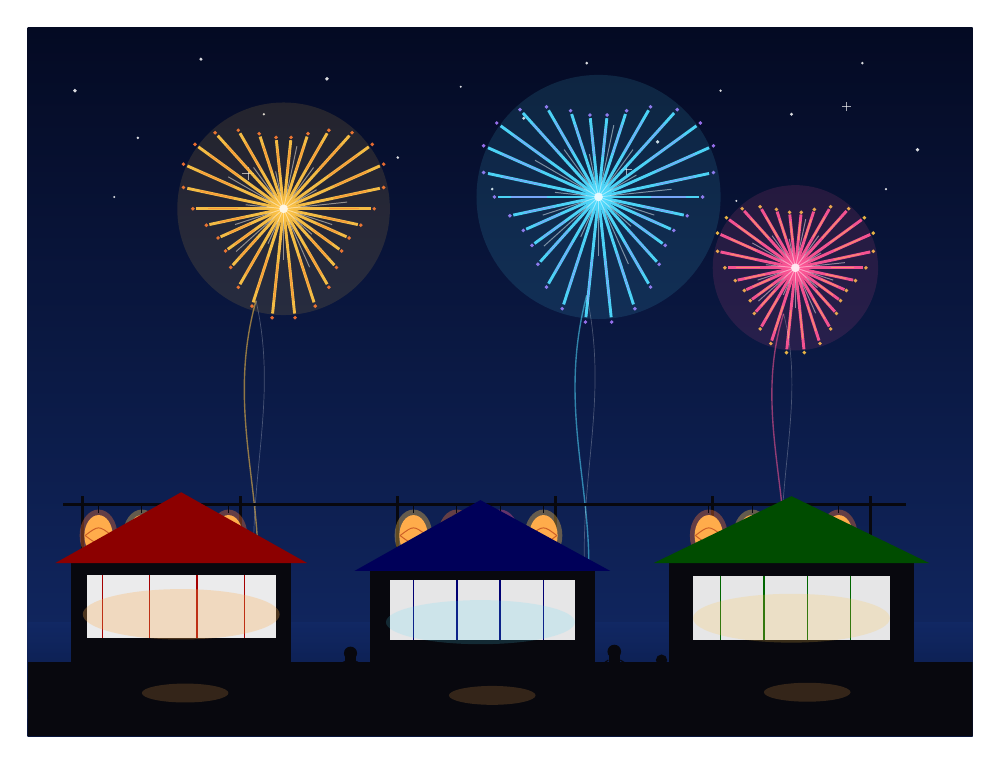
\begin{tikzpicture}[x=1cm,y=1cm]
\clip (0,0) rectangle (12,9);

\definecolor{nightA}{RGB}{4,10,35}
\definecolor{nightB}{RGB}{9,23,72}
\definecolor{nightC}{RGB}{18,42,104}
\definecolor{gold}{RGB}{255,196,70}
\definecolor{orange}{RGB}{255,116,48}
\definecolor{pink}{RGB}{255,86,150}
\definecolor{cyan}{RGB}{80,220,255}
\definecolor{violet}{RGB}{165,120,255}
\definecolor{lantern}{RGB}{255,172,75}
\definecolor{shadow}{RGB}{8,8,14}

\shade[top color=nightA,middle color=nightB,bottom color=nightC] (0,0) rectangle (12,9);

\foreach \x/\y/\r in {
0.6/8.2/0.025,1.4/7.6/0.018,2.2/8.6/0.022,3.0/7.9/0.016,
3.8/8.35/0.025,4.7/7.35/0.018,5.5/8.25/0.015,6.3/7.85/0.02,
7.1/8.55/0.018,8.0/7.55/0.024,8.8/8.2/0.016,9.7/7.9/0.02,
10.6/8.55/0.018,11.3/7.45/0.024,1.1/6.85/0.014,5.9/6.95/0.018,
9.0/6.8/0.014,10.9/6.95/0.016}
  \fill[white,opacity=0.85] (\x,\y) circle (\r);

\foreach \x/\y/\s in {2.8/7.15/0.08,7.6/7.2/0.07,10.4/8.0/0.06}
{
  \draw[white,opacity=0.65,line width=0.25pt] (\x-\s,\y) -- (\x+\s,\y);
  \draw[white,opacity=0.65,line width=0.25pt] (\x,\y-\s) -- (\x,\y+\s);
}

\newcommand{\firework}[5]{
  \foreach \a in {0,12,...,348}{
    \pgfmathsetmacro{\len}{#3*(0.82+0.18*sin(3*\a))}
    \draw[#4,opacity=0.95,line width=1.05pt]
      (#1,#2) -- ++(\a:\len);
    \draw[#5,opacity=0.55,line width=0.45pt]
      (#1,#2) ++(\a:{0.52*\len}) -- ++(\a:{0.35*\len});
    \fill[#5,opacity=0.9] (#1,#2) ++(\a:{1.04*\len}) circle (0.025);
  }
  \foreach \a in {6,30,...,342}{
    \pgfmathsetmacro{\len}{#3*(0.48+0.14*cos(5*\a))}
    \draw[white,opacity=0.5,line width=0.35pt]
      (#1,#2) -- ++(\a:\len);
  }
  \fill[white,opacity=0.95] (#1,#2) circle (0.055);
  \fill[#4,opacity=0.12] (#1,#2) circle (#3);
}

\firework{3.25}{6.7}{1.35}{gold}{orange}
\firework{7.25}{6.85}{1.55}{cyan}{violet}
\firework{9.75}{5.95}{1.05}{pink}{gold}

\foreach \x/\h/\c in {2.9/2.2/gold,7.1/2.4/cyan,9.6/1.7/pink}{
  \draw[\c,opacity=0.55,line width=0.5pt] (\x,1.7) .. controls (\x+0.15,3.0) and (\x-0.4,4.1) .. (\x,4.8+\h/3);
  \draw[white,opacity=0.25,line width=0.25pt] (\x,1.7) .. controls (\x-0.15,3.2) and (\x+0.3,4.2) .. (\x,4.8+\h/3);
}

\shade[top color=nightC,bottom color=nightA,opacity=0.65] (0,0) rectangle (12,1.45);
\foreach \x/\w/\o in {0.4/1.3/0.10,2.0/1.5/0.14,4.0/1.2/0.10,6.0/1.7/0.16,8.4/1.4/0.12,10.2/1.7/0.15}{
  \fill[gold,opacity=\o] (\x,0.35) ellipse ({\w} and 0.13);
}

\fill[shadow] (0,0) rectangle (12,0.95);

\foreach \x in {0.7,2.7,4.7,6.7,8.7,10.7}{
  \draw[shadow,line width=1pt] (\x,0.95) -- (\x,3.05);
}

\draw[shadow,line width=1.1pt] (0.45,2.95) -- (11.15,2.95);

\foreach \x/\c in {0.9/orange,1.45/gold,2.0/pink,2.55/orange,4.9/gold,5.45/orange,6.0/pink,6.55/gold,8.65/orange,9.2/gold,9.75/pink,10.3/orange}{
  \fill[\c,opacity=0.36] (\x,2.55) ellipse (0.24 and 0.33);
  \fill[lantern] (\x,2.55) ellipse (0.18 and 0.26);
  \draw[orange!80!black,line width=0.35pt] (\x-0.17,2.55) .. controls (\x,2.68) .. (\x+0.17,2.55);
  \draw[orange!80!black,line width=0.35pt] (\x-0.17,2.55) .. controls (\x,2.42) .. (\x+0.17,2.55);
  \draw[shadow,line width=0.35pt] (\x,2.84) -- (\x,2.95);
}

\fill[shadow] (0.55,0.9) rectangle (3.35,2.25);
\fill[red!55!black] (0.35,2.2) -- (1.95,3.1) -- (3.55,2.2) -- cycle;
\fill[white,opacity=0.92] (0.75,1.25) rectangle (3.15,2.05);
\foreach \x in {0.95,1.55,2.15,2.75}
  \draw[red!65!black,line width=0.5pt] (\x,1.25) -- (\x,2.05);
\fill[lantern,opacity=0.28] (1.95,1.55) ellipse (1.25 and 0.32);

\fill[shadow] (4.35,0.9) rectangle (7.2,2.15);
\fill[blue!35!black] (4.15,2.1) -- (5.75,3.0) -- (7.4,2.1) -- cycle;
\fill[white,opacity=0.9] (4.6,1.22) rectangle (6.95,1.98);
\foreach \x in {4.9,5.45,6.0,6.55}
  \draw[blue!45!black,line width=0.5pt] (\x,1.22) -- (\x,1.98);
\fill[cyan,opacity=0.16] (5.75,1.45) ellipse (1.2 and 0.28);

\fill[shadow] (8.15,0.9) rectangle (11.25,2.25);
\fill[green!30!black] (7.95,2.2) -- (9.7,3.05) -- (11.45,2.2) -- cycle;
\fill[white,opacity=0.9] (8.45,1.22) rectangle (10.95,2.03);
\foreach \x in {8.8,9.35,9.9,10.45}
  \draw[green!40!black,line width=0.5pt] (\x,1.22) -- (\x,2.03);
\fill[gold,opacity=0.2] (9.7,1.5) ellipse (1.25 and 0.31);

\foreach \x/\y/\s in {
1.0/0.8/0.58,1.55/0.74/0.48,2.45/0.78/0.5,3.25/0.75/0.47,
4.1/0.77/0.52,4.8/0.73/0.44,5.55/0.76/0.5,6.45/0.74/0.46,
7.45/0.78/0.54,8.05/0.72/0.45,8.9/0.77/0.5,9.65/0.74/0.48,
10.4/0.78/0.53,11.1/0.75/0.46}
{
  \fill[shadow] (\x,\y+0.55*\s) circle (0.16*\s);
  \fill[shadow] (\x-0.13*\s,\y+0.13*\s) rectangle (\x+0.13*\s,\y+0.52*\s);
  \draw[shadow,line width={1.0*\s pt}] (\x-0.13*\s,\y+0.12*\s) -- (\x-0.32*\s,\y-0.25*\s);
  \draw[shadow,line width={1.0*\s pt}] (\x+0.13*\s,\y+0.12*\s) -- (\x+0.30*\s,\y-0.25*\s);
  \draw[shadow,line width={0.8*\s pt}] (\x-0.14*\s,\y+0.35*\s) -- (\x-0.38*\s,\y+0.18*\s);
  \draw[shadow,line width={0.8*\s pt}] (\x+0.14*\s,\y+0.35*\s) -- (\x+0.38*\s,\y+0.2*\s);
}

\foreach \x/\y in {2.0/0.55,5.9/0.52,9.9/0.56}{
  \fill[lantern,opacity=0.18] (\x,\y) ellipse (0.55 and 0.12);
}

\end{tikzpicture}
\end{document}
